\chapter{Implementation}
\label{cha:Implementation}
The final implementation was done in Java, and was built on top of the AIM simulator codebase. All class diagrams were created using the `IntelliJ IDEA 15.0.3' internal diagram tool. Figure \ref{fig:classDiagramKey} provides a key for understanding these diagrams.

\begin{figure}[htb]
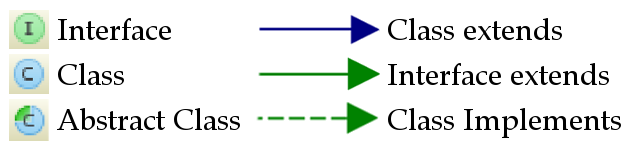
\includegraphics[width=\textwidth]{classDiagrams/classDiagramKey.png}
\caption{Key for the class diagrams in this report.}
\label{fig:classDiagramKey}
\end{figure}

\section{Generalising the Codebase}
\label{sec:Generalising the Codebase}
The use of the AIM codebase was a project restriction imposed for research purposes. By working with the AIM simulator codebase I could learn how easy it is to work with, and analyse whether or not it would be a good codebase to continue expanding upon for future AV projects. Each simulator built for this project works alongside the AIM simulators, whilst being completely independent. The project: \citetitle{Milligan2017} \citep{Milligan2017}, was also required to be built using AIM. In addition both projects had to work alongside each other using the same codebase. To make sure that code coupling was reduced as much as possible, I worked closely with their project lead to generalise the codebase, breaking out useful shared features so that they could be accessed by all simulator types. The final code can be found at \url{https://github.com/CallumHewitt/AVSimulatorProject} \citep{Codebase}. Breaking out the code like this satisfied requirements \emph{NS.11} and \emph{NS.12}.

Appendix \ref{sec:Generalising the Codebase Appendix} provides detailed coverage of the changes made to the AIM codebase.

\begin{tabular}{|c|c|c|}
\hline
Requirement Code & Achieved? \\
\hline
NS.11 & \cellcolor{green} \cmark \\
NS.12 & \cellcolor{green} \cmark \\ 
\hline
\end{tabular}

\section{Merge Schemes}
\label{sec:Merge Schemes}
The AMM protocol implementation was developed by examining the original AIM code and creating a modified version applicable to merges. Because the two systems are so similar, much of the code was duplicated. This could be refactored out a later date, but during development having full control over the actions taken by a vehicle without having to compromise to allow AIM to work correctly was very useful. In the end, despite this approach there were significant issues with the system. Despite using very similar approaches to AIM, almost identical in areas, vehicles would continue to arrive early to their reserved times and vehicles would also collide consistently at intersections. The reasons for these errors are described in more detail in Section \ref{sec:Simulation}.

To correctly implement the AMM system much of the fundamental generalised code that the system was built upon would have had to be replicated or rewritten to ensure that the system was working accurately. Because of this, and due to time constraints, a full version of the AMM system was not implemented. As such requirement \emph{FS.81} was not satisfied. As an alternative, a modified version of the AIM simulator was developed. In this version the AIM simulator was restricted to only spawn vehicles from the south and west roads, with each vehicle's destination set to the east road. This effectively mimicked an AMM system with a 90\degree merge angle.

The QMM system was implemented as a replacement for a fully implemented AMM system. The system was expected to have good performance, possibly rivalling that of the AMM system. We expected the queue system to act more fairly to each lane, distributing the vehicle load evenly. The system was also simpler to implement than the AMM system, and despite issues surrounding some of the generalised methods, the system was fully implemented. With QMM implemented, we now had a system which could be used to analyse how the merge factors, such as merge angle, speed limits and lead in distances, affect a system. We can also compare the performance of the AMM and QMM protocols.

The QMM system was implemented with a distance limit of 150\si{m}. Vehicles further than this distance cannot be added to the queue.

The original plan was to compare a centralised system with a decentralised solution, based on the work from VanMiddlesworth \citep{VanMiddlesworth2008}. However, this was never implemented due to time constraints. As such requirement \emph{FS.91} was not satisfied.

\begin{tabular}{|c|c|c|}
\hline
Requirement Code & Achieved? \\
\hline
FS.81 & \cellcolor{red} \xmark \\
FS.91 & \cellcolor{red} \xmark \\
\hline
\end{tabular}

\section{Simulation}
\label{sec:Simulation}
Each simulation consists of multiple interacting agents, which makes it a difficult problem to implement. Using some of the generalised AIM classes helped to reduce the amount of time it took to implement these components. However, using AIM did introduce some complications and parts of the code had to be rewritten to adjust for this.

\subsection{Drivers}
\label{subsec:Drivers}
Driver agents are responsible for manipulating the vehicles in the simulation. They make requests to centralised merge managers and act upon the responses they are given. Each driver acts as a finite state machine, performing specific sets of actions for each state. Vehicles and Drivers both extend from generalised Vehicle and Driver classes containing useful functions for following lanes, turning and determining distances. However, some of these methods proved to be flawed.

One of the main issues was the assumption that lanes and roads will always meet at 90\degree. This caused a number of small issues throughout development, but one key problem was turning. A turn through an intersection in the AIM simulator is done by forcing the vehicle to point to a coordinate further down the lane the vehicle is following. This point is always exactly the same distance away from the vehicle, such that when the vehicle reaches a corner, and the lane it's following changes, the vehicle will turn towards that point gradually. This distance proved too much for some merges, and resulted in the vehicle making turns too gradually. This was fixed by setting the turn distance to always be the distance from the point at which the vehicle enters the merge zone, to the merge zone exit. The target point would also always lie in the centre of the target lane. This caused merging vehicles to turn more tightly, freeing up the lane for more vehicles. Figure \ref{fig:turning} shows how these turns work.

\begin{figure}[htb]
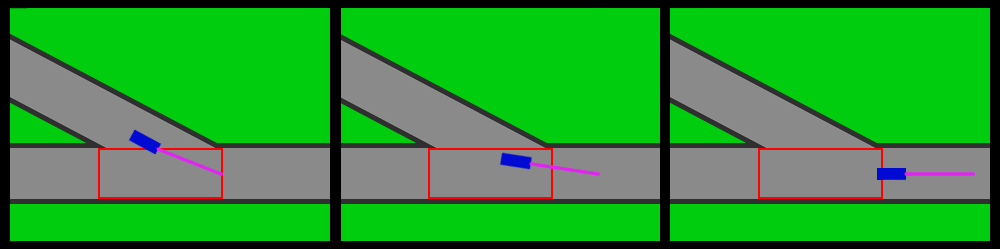
\includegraphics[width=\textwidth]{implementationDiagrams/turning.png}
\caption{A diagram indicating how turning works through a merge. Red indicates the Merge Zone, Blue indicates a vehicle, Pink indicates the aiming distance and the point the vehicle is turning towards.}
\label{fig:turning}
\end{figure}

Another problem came about due to collisions. AIM had provided a method called \emph{dontHitCarInFront} which calculates the distance from the vehicle to the vehicle in front and then takes action to avoid a collision, slowing down if necessary. This method turns out to not be completely effective, particularly at high speeds. Even within the original AIM simulations, vehicles collide. Due to time constraints collision detection was removed from the project, as fixing the issue would have required in depth analysis of core methods. As such requirement \emph{FS.162} was not fulfilled. As far as I can tell, no collisions take place within the QMM merge zone, as it should be almost impossible, but without having a check in place this cannot be said for certain. The AIM protocol also avoids collisions in the merge zone by switching to `acceleration profiles' instead of using the \emph{dontHitVehicleInFront} method.

\subsection{Merge Managers}
\label{subsec:Merge Managers}
The role of a merge manager is to take requests from drivers and provide responses, controlling the flow of traffic through the merge zone. They were heavily influenced by the approaches taken by AIM. The AMM merge manager replicated much of the intersection manager code introduced by AIM. At a later date this could be refactored to reduce duplication, but this would most likely also require changes to Driver and Vehicle, as each type of merge manager is built to deal with different types of vehicles and drivers.

The final implementation of a merge manager, the \emph{QueueV2IManager}, is designed similarly to AIM's \emph{V2IIntersectionManager}, however much of the code is original and far simpler. This merge manager effectively just manages a queue and alerts vehicles when they are at the front of said queue. The AIM system is more complex, requiring the merge manager to monitor reservations and time the arrival of vehicles as they arrive. The AIM system relies very heavily on each vehicle arriving at their stated time and fails to handle vehicles well if they don't.

\subsection{Map}
\label{subsec:Map}
The simulation map stores all of the spawn points, lanes and merge managers for the simulation.

By using some of the generalised components for calculating distances, creating the map was relatively straightforward, however, there were some components that failed to work as intended. The original AIM system assumes that every road meets at 90\degree and as such some methods were inappropriate for when lanes meet at other angles. One example of this is the no vehicle zone at the beginning of each lane. This zone stops multiple vehicles from spawning on top of each other. The original implementation calculated a \emph{Rectangle2D} at the beginning of each lane, which works fine when lanes are at 90\degree. For my no vehicle zones, I had to define a path around the start of each merge lane and create a shape from that. This more complicated approach was necessary due to the angles at which the merge lane can meet the target lane. 

The map also controls the spawn points creating the vehicles. Most spawning behaviours were based on the AIM spawn points. However, to enable consistent testing we wanted to be able to repeat the experiment with the same vehicles over and over again. To do this I created a new vehicle spawn type that uses a JSON file to spawn vehicles. The file contains an array of vehicle specification and spawn time pairs. The spawner reads this data in and spawns a vehicle with the given specification at the indicated time. I also implemented this type of spawner into the AIM system. This means that direct comparisons between the performance of AIM and the QMM protocol are now possible.

\subsection{Simulation Control}
\label{subsec:Simulation Control}
The simulator itself is reponsible for triggering and monitoring the actions of each component of the simulation. It delivers messages between merge managers and vehicles and moves vehicles through the simulation according to their specified velocities and headings. The simulator controller satisfies requirements \emph{FS.12}, \emph{FS.13}, \emph{FS.22}, \emph{FS.32}, \emph{FS.42}, \emph{FS.71}, \emph{FS.73}, \emph{NS.3}, \emph{NS.4} and \emph{NS.8} by managing all of the component in the simulation and producing results.

\begin{tabular}{|c|c|c|}
\hline
Requirement Code & Achieved? \\
\hline
FS.12 & \cellcolor{green} \cmark \\
FS.13 & \cellcolor{green} \cmark \\
FS.22 & \cellcolor{green} \cmark \\
FS.32 & \cellcolor{green} \cmark \\
FS.42 & \cellcolor{green} \cmark \\
FS.71 & \cellcolor{green} \cmark \\
FS.73 & \cellcolor{green} \cmark \\
FS.162 & \cellcolor{red} \xmark \\
NS.3 & \cellcolor{green} \cmark \\
NS.4 & \cellcolor{green} \cmark \\
NS.8 & \cellcolor{green} \cmark \\
\hline
\end{tabular}

\section{Results Production}
\label{sec:Results Production}
In order to provide results Vehicle objects were provided with fields to store their statistics. These fields were:

\begin{itemize}
\item Delay
\item Final Velocity
\item Maximum Velocity
\item Minimum Velocity
\item Final X Position
\item Final Y Position
\item Start Time
\item Finish Time
\item Starting Road
\end{itemize}

These fields were implemented in both AIM and Merge vehicles. This allows for a comparison between AIM and QMM protocols at 90\degree.

To calculate the delay the simulator first simulates each vehicle specification for both the merge and target road. The completion times for each specification are recorded and then used to calculate the effect the merge protocol had on each vehicle. The start time and starting roads are initialised in each vehicle when they are created by their spawn point. The maximum and minimum velocities are dealt with after the \emph{moveVehicles} method in the simulator. The simulator compares the current velocity of the vehicle to its stored maximum and minimum velocity and updates as necessary. The finishing variables are dealt with when the simulator removes them from the simulation and adds them to the completed vehicle store. 

Maximum acceleration and deceleration measurements were not implemented, and as such requirements \emph{FS.6a}, \emph{FS.6b}, \emph{FS.6d} and \emph{FS.6e} were not satisfied. All other requirements connected to \emph{FU.6} and \emph{NS.7} were satisfied. AIMs current design uses the maximum deceleration for each vehicle as they approach the merge zone, braking at the last moment as aggressively as the vehicle's specification allows. This obviously makes maximum acceleration and deceleration measurements pointless. In real life braking profiles like this won't provide the most comfortable ride to passengers, and it also means that vehicles cannot pre-emptively slow down to maintain momentum whilst other vehicles to move through the merge. Further work could be done to expand both the AIM and Queue protocols to allow for pre-emptive acceleration profiles like these.

The results can be saved to a CSV file containing the throughput, maximum delay, mean delay and minimum delay of the system. There are also results for each vehicle. In addition to the list above, each result contains the vehicle's

\begin{itemize}
\item VIN
\item Starting Road
\item Vehicle Specification Name
\end{itemize}

\begin{tabular}{|c|c|c|}
\hline
Requirement Code & Achieved? \\
\hline
FS.62 & \cellcolor{green} \cmark \\
FS.63 & \cellcolor{green} \cmark \\
FS.64 & \cellcolor{green} \cmark \\
FS.65 & \cellcolor{green} \cmark \\
FS.66 & \cellcolor{green} \cmark \\
FS.67 & \cellcolor{green} \cmark \\
FS.68 & \cellcolor{green} \cmark \\
FS.69 & \cellcolor{green} \cmark \\
FS.6a & \cellcolor{red} \xmark \\
FS.6b & \cellcolor{red} \xmark \\
FS.6c & \cellcolor{green} \cmark \\
FS.6d & \cellcolor{red} \xmark \\
FS.6e & \cellcolor{red} \xmark \\
NS.7 & \cellcolor{green} \cmark \\
\hline
\end{tabular}

\section{GUI}
\label{sec:GUI}
The GUI for the project was built using Java Swing, extending the existing GUI. New simulator types are given a separate tab in the application with their own simulator setup and a display screen. The display screen can be modified for each simulation type, showing the relevant information for that simulation. We moved away from the AIM graphical implementation to a \emph{StatScreen} implementation which shows information in text format instead. The S2S simulations display the current simulation time, number of completed vehicles and throughput. They also display two tables, one containing information about the vehicles currently in the simulation, and another for vehicles that have left the simulation. Figure \ref{fig:s2sSimScreen} shows the simulation screen for S2S merges.

\begin{sidewaysfigure}[p]
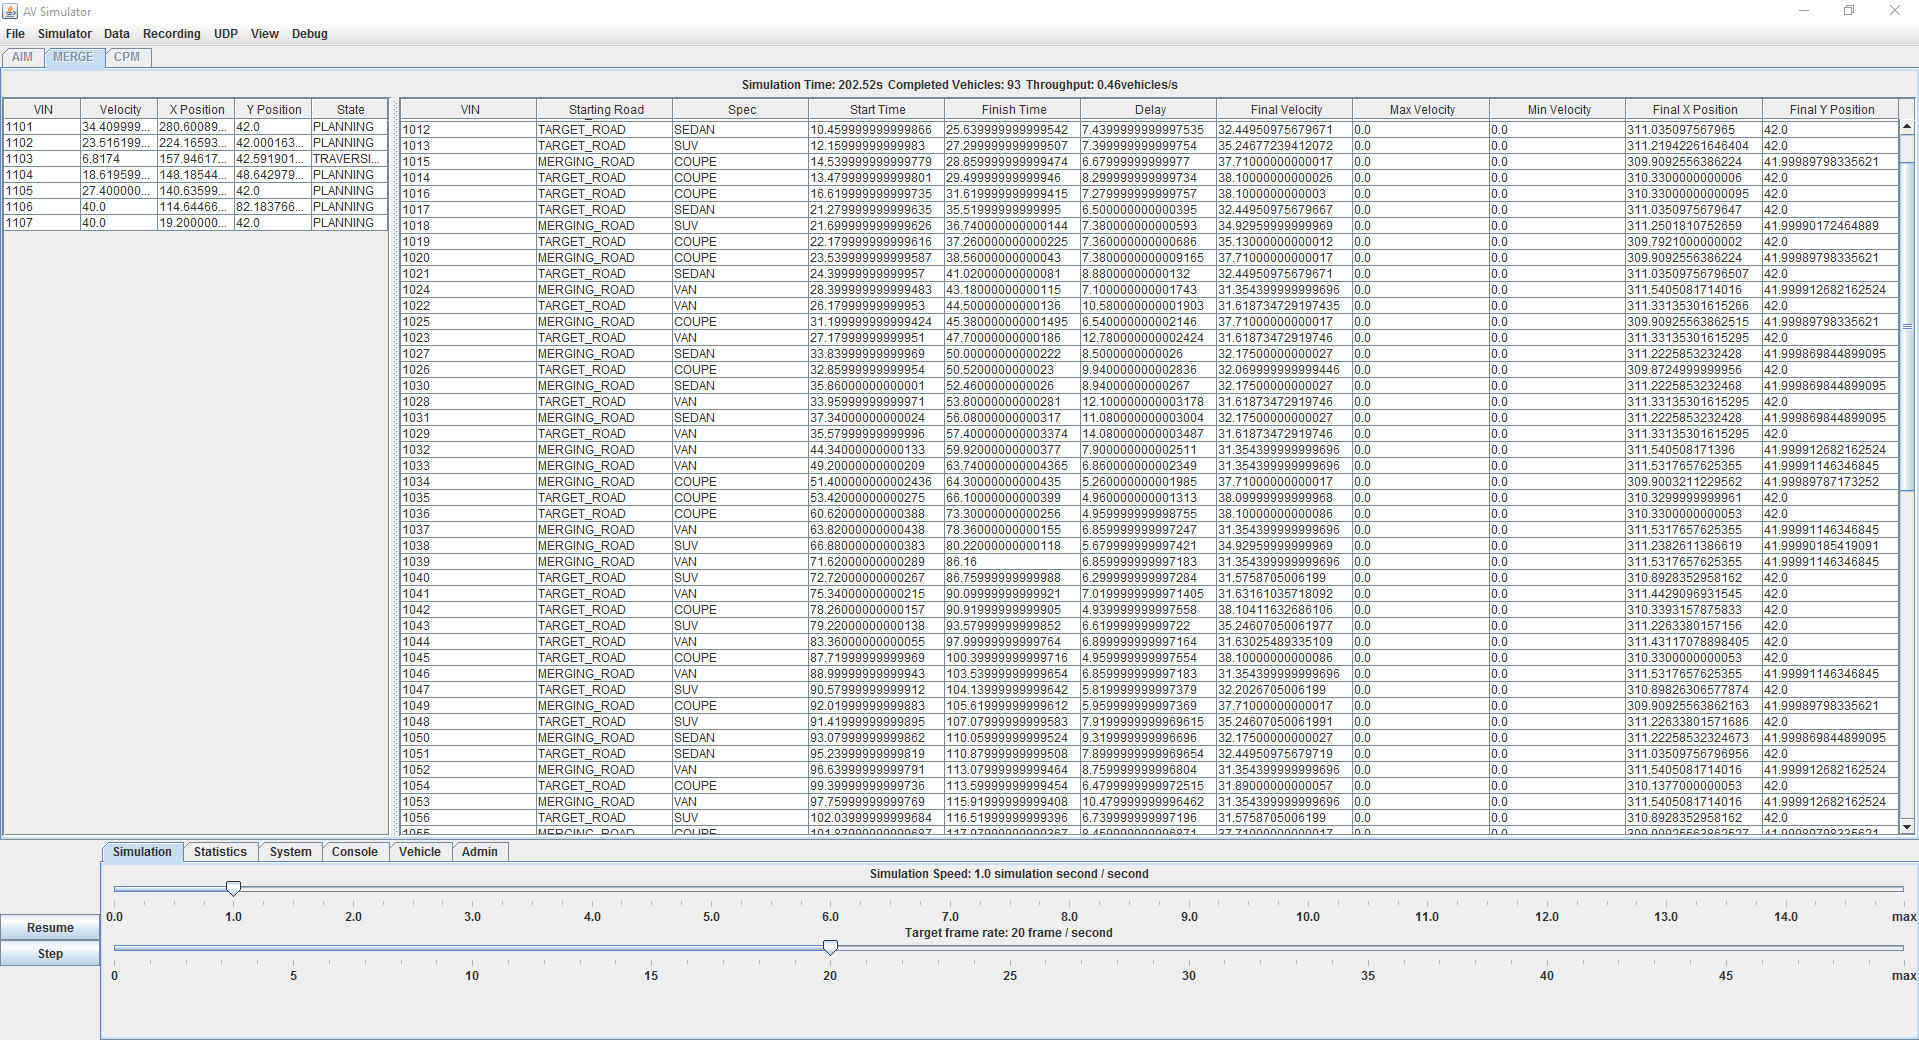
\includegraphics[width=\textwidth]{screenshots/s2sSimulationScreen.png}
\caption{The simulation screen for the S2S merge screen}
\label{fig:s2sSimScreen}
\end{sidewaysfigure}

Functional requirements \emph{FS.82} and \emph{FS.92} were not fully implemented as the AIM-like simulations and Decentralised simulations were never implemented in a fully working form. \emph{FS.161} was also never implemented due to the removal of collision detection from simulations. All other GUI requirements were completed. All other requirements were completed.

In order to enable repeat experiments with the same vehicles spawning at the same time, the GUI needed to support the uploading of merge schedule JSON files to the spawn points. This was implemented using \emph{JFileChooser}. I also added an extra feature to the merge setup panel which allows users to generate spawn schedule files for a specific time period at a specified traffic level. This enables users to generate schedules without having access to the codebase.

\begin{tabular}{|c|c|c|}
\hline
Requirement Code & Achieved? \\
\hline
FS.11 & \cellcolor{green} \cmark \\
FS.21 & \cellcolor{green} \cmark \\
FS.31 & \cellcolor{green} \cmark \\
FS.41 & \cellcolor{green} \cmark \\
FS.51 & \cellcolor{green} \cmark \\
FS.61 & \cellcolor{green} \cmark \\
FS.72 & \cellcolor{green} \cmark \\
FS.82 & \cellcolor{red} \xmark \\
FS.92 & \cellcolor{red} \xmark \\
FS.101 & \cellcolor{green} \cmark \\
FS.111 & \cellcolor{green} \cmark \\
FS.121 & \cellcolor{green} \cmark \\
FS.131 & \cellcolor{green} \cmark \\
FS.141 & \cellcolor{green} \cmark \\
FS.151 & \cellcolor{green} \cmark \\
FS.161 & \cellcolor{red} \xmark \\
NS.1 & \cellcolor{green} \cmark \\
NS.2 & \cellcolor{green} \cmark \\
NS.5 & \cellcolor{green} \cmark \\
NS.6 & \cellcolor{green} \cmark \\
\hline
\end{tabular}

\section{Maintainability and Testing}
\label{sec:Testing}

\subsection{Maintainability}
\label{subsec:Maintainability}
The separability imposed between AIM, Merge and Generalised classes allows developers to create new simulations quickly, without having concerns over the effect they'll have on existing work. In general, as long as the developers extend and modify certain key classes they can create without worry. For example, new developers will have to create a new \emph{SimSetupPanel} and \emph{SimViewer} panel in order for their simulation to appear in the GUI. The separability isn't perfect, there are some instances where AIM specific classes are used by Merge (mainly in the implementation of AMM), but in general most of the classes are broken out correctly, satisfying requirement \emph{NS.9}.

In terms of maintaining existing code, the prospects are quite good. The  majority of the complex code is documented using JavaDocs, and comments, satisfying requirement \emph{NS.10}. Once familiar with the codebase, it is relatively easy to find the files you are aiming to change. Some sections are quite complex however. Many AIM components are tightly coupled, particularly surrounding the I2V managers and reservation classes. These areas use callback interfaces that result in confusion over the role of each class. Refactoring this out would be hard, as there isn't really a perfect solution in this instance, but it could be done with further development time. The separability of the different simulators also comes at a cost in terms of class structure complexity. The changes made to the vehicle classes in section \ref{sec:Generalising the Codebase} should indicate how complex some of the class structures have become.

The main problem with the codebase surrounds the core generalised code. Because the system is based on AIM development can be difficult to attempt to use the system for something beyond the original specification, such as using lanes that don't meet at 90\degree. These problems have already been described in Section \ref{sec:Simulation}.

\subsection{Unit Testing}
\label{subsec:Unit Testing}
Unit tests were mostly used to ensure getter and setter methods worked as expected. However, some unit tests were used to verify the behaviour of classes. To do this I used Mockito \citep{MockitoWebsite} to mock the behaviour of objects used by the test class so that I could prompt the test class into producing the expected results. Mockito was particularly useful in dealing with the components with high coupling.

\subsection{Integration Tests}
\label{subsec:Integration Tests}
Integration tests were the most useful tests I used. They allowed me to find and remove problems with the simulators by observing how the map, vehicles, drivers and simulator objects interacted together, as this was usually where most of the errors were occuring. These tests also allowed me to identify key errors with the AIM simulator's approach that were causing problems with the AMM.

\begin{tabular}{|c|c|c|}
\hline
Requirement Code & Achieved? \\
\hline
NS.9 & \cellcolor{green} \cmark \\
NS.10 & \cellcolor{green} \cmark \\
\hline
\end{tabular}